\documentclass[11pt, a4paper]{article}

% --- 通用导言区 (Universal Preamble Block) ---
% 页面布局设置
\usepackage[a4paper, top=2.5cm, bottom=2.5cm, left=2cm, right=2cm]{geometry}
% 使用 ctex 宏包来处理中文支持（在 XeLaTeX/LuaLaTeX 下工作良好）
\usepackage[UTF8]{ctex}

% 图片支持
\usepackage{graphicx}
% 允许在非浮动环境中使用 \captionof
\usepackage{caption}
% 让图注左对齐
\captionsetup{justification=raggedright,singlelinecheck=false}
% 全局左对齐（避免两端对齐），使用 ragged2e 提供更好的断行
\usepackage{ragged2e}
% 在文档开始时启用 \RaggedRight（放在导言区以避免错误）
\AtBeginDocument{\RaggedRight}

% 列表样式修正
\usepackage{enumitem}
\setlist[itemize]{label=-}

% 数学公式包
\usepackage{amsmath}

% --- 用户指南: 如何插入图片 ---
% 1. 在本地编译时，请确保您安装了 'graphicx' 宏包。
% 2. 取消下面这一行代码的注释（去掉行首的 %）：
% \usepackage{graphicx}
% 3. 在下文中找到 "figure" 环境，将 \framebox{...} 部分替换为 \includegraphics 命令。

\title{Lab 3}
\author{姓名：黄瑞颀； 学号：2024531064}


\begin{document}

\maketitle
\newpage
\section{数据处理与线性拟合}
\begin{figure}[htbp]
    \centering
    \begin{minipage}[t]{0.48\textwidth}
    首先我们知道ln（x）函数的定义域是正数，所以我们首先过滤掉表格中的非正数只保留正数，并且将$I_{d}$数据取对数，得到如下数据表格：
        \centering
        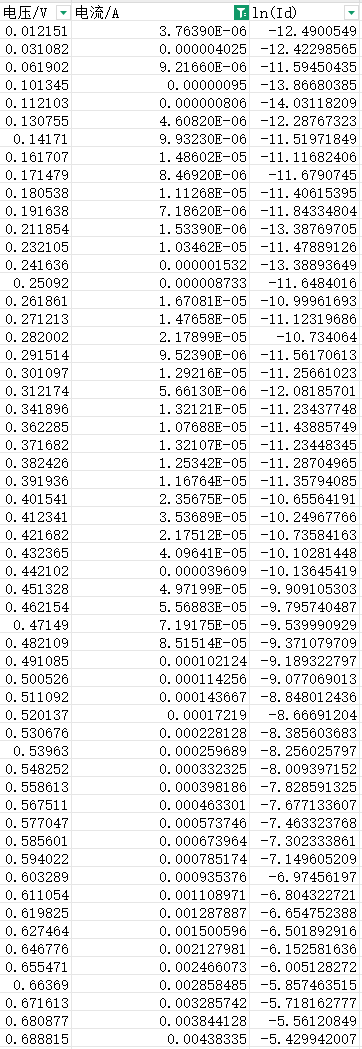
\includegraphics[width=0.7\linewidth]{lab3_1_data.png}
        \captionof{figure}{$ln(I_{d})$ 与 $V_{d}$ 的数据表格}
        \label{fig:lab3_1_data}
    \end{minipage}\hfill
    \begin{minipage}[t]{0.48\textwidth}
        对这些处理过后的数据进行可视化，其中图表的纵轴是$ln(I_{d})$,横轴是$V_{d}$，并对数据S进行线性拟合，得到右图：
        \vspace{0pt}
        \centering
        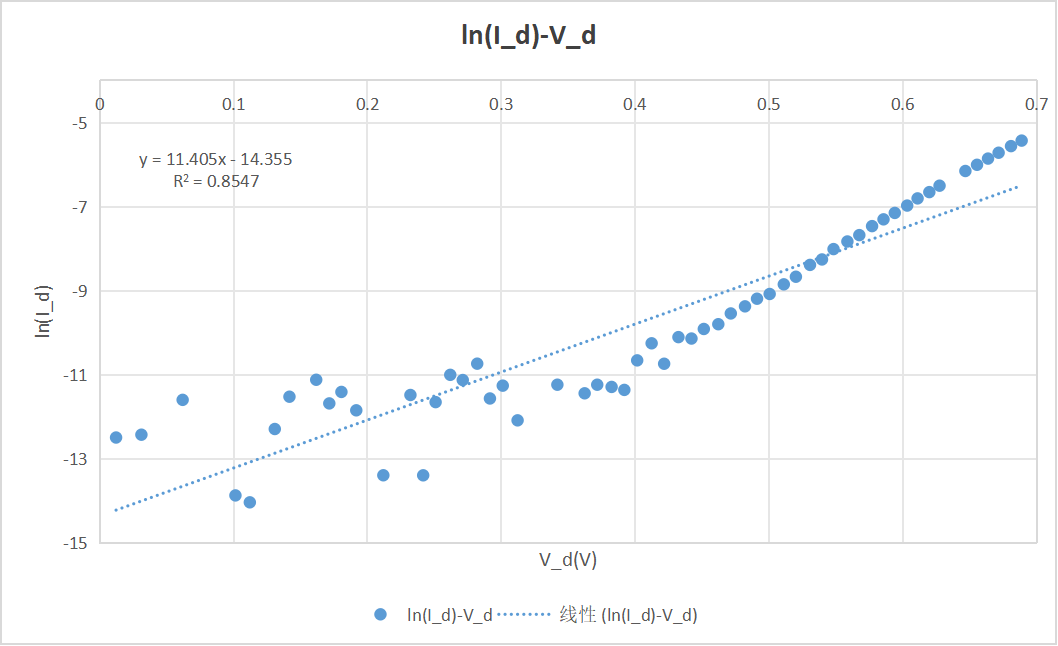
\includegraphics[width=0.95\linewidth]{lab3_1.png}
        \captionof{figure}{$ln(I_d)$ 对 $V_d$ 的关系及拟合}
        \label{fig:lab3_1}
        \vspace{0.1em}
    经过拟合发现$R^2 = 0.8547$，线性拟合效果很差，在大约 $V_{d}<0.4V$ 的情况下，或许由于仪器分辨率限制，数据非常不稳定。因此我们截取$V_{d}\geq 0.4V$的数据进行分析，其数据表格如下：\\
        \centering
        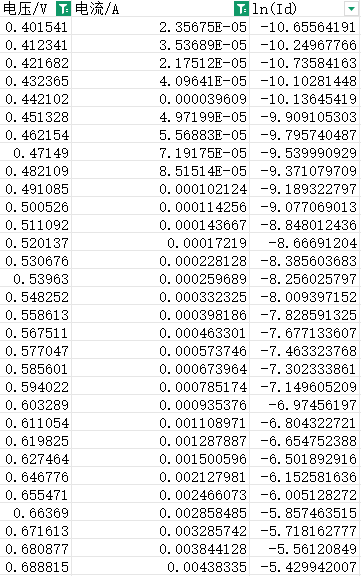
\includegraphics[width=0.65\linewidth]{lab3_2_data.png}
        \captionof{figure}{$ln(I_{d})$ 与 $V_{d}$ 的部分数据表格}
        \label{fig:lab3_2_data}
        \vspace{0.1em}
    \end{minipage}
\end{figure}

\newpage
\begin{figure}[htbp]
    \centering
    \begin{minipage}[t]{0.48\textwidth}
    对上述的$V_{d}\geq 0.4V$的数据绘图，得到下图:\
        \RaggedRight
        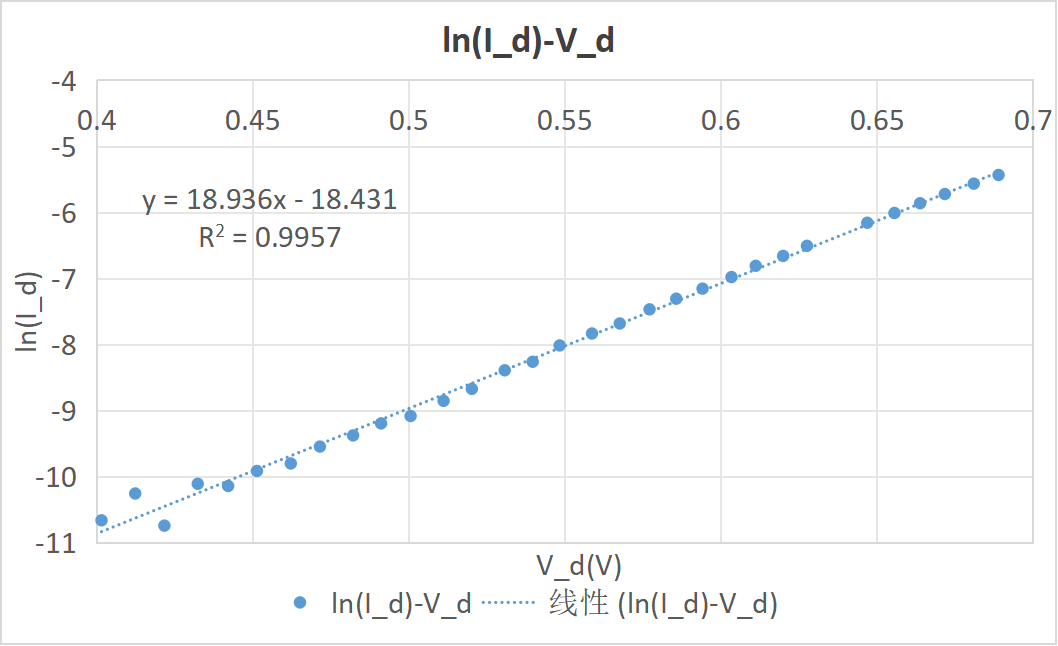
\includegraphics[width=1.0\linewidth]{lab3_2.png}
        \captionof{figure}{$ln(I_{d})$ 与 $V_{d}$ 的优秀数据表格}
        \label{fig:lab3_2}
    通过拟合方程可以得出：
    $$
    \frac{1}{nV_{T}}=18.936
    $$
    $$
    ln(I_{s})=-18.431
    $$

    由 $V_{T}=25.3mV=0.0253V$ 可得：
    $$
    n=2.087
    $$
    $$
    I_{s}=9.897\times10^{-9}A
    $$
    \end{minipage}\hfill
    \begin{minipage}[t]{0.48\textwidth}
    \section{MATLAB 自定义方程验证}
    因为删除了一部分数据，因此可以用 Matlab 的曲线拟合器，通过自定义方程拟合的方式，检验上述数据的准确性。

    在 Matlab 中，拟合类型选择为自定义方程，方程形式设置为：
    $$
    y=a\cdot[e^{bx}-1]
    $$
    即：
    $$
    I_{d}=a\cdot[e^{bV_{d}}-1]
    $$

    拟合结果如下图所示：
    \end{minipage}
\end{figure}
% --- 图片占位符 3 ---
% [如何修改为真实图片]:
% 替换下面的 \framebox 代码块为: \includegraphics[width=0.9\textwidth]{您的Matlab截图.jpg}
    \RaggedRight
        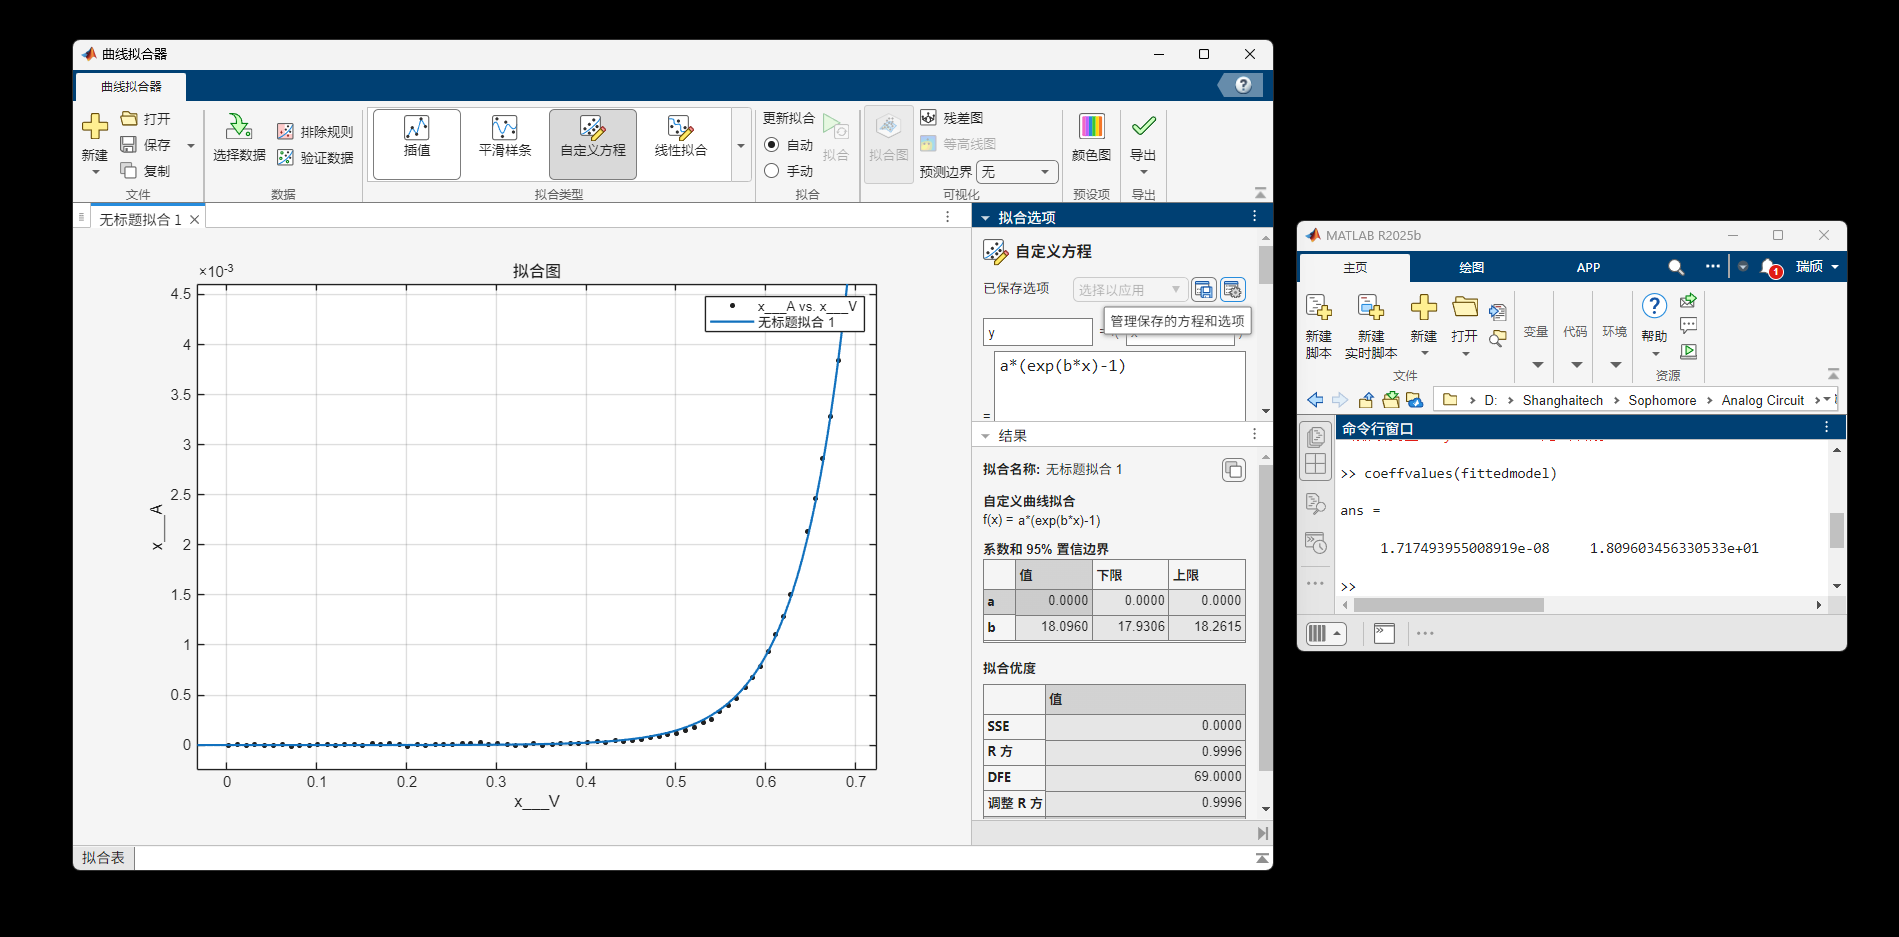
\includegraphics[width=1.0\linewidth]{fitted_model.png}
        \captionof{figure}{matlab 自定义方程拟合结果}
    \label{fig:fitted_model}
  根据 Matlab 拟合结果：
    $$
    a=1.717\times10^{-8}
    $$
    $$
    b=18.1
    $$

    即方程为：$I_{d}=1.717\times10^{-8}[e^{18.1x}-1]$

    所以可以计算出：

    \begin{align*}
        I_{s} &= a = 1.717\times10^{-8}A \\
        n &= \frac{1}{b\cdot V_{T}} = \frac{1}{18.1\times 25.3\times 10^{-3}} = 2.18
    \end{align*}





\section{结论}
通过对实验数据的处理与分析，我们得到了二极管的反向饱和电流$I_{s}$和理想因子$n$的近似值。具体结果如下：
\begin{itemize}
    \item 最终结果：
    \begin{itemize}
        \item 反向饱和电流$I_{s} \approx 9.897 \times 10^{-9}A$
        \item 理想因子$n \approx 2.087$
    \end{itemize}
\end{itemize}
总体来看，实验数据与理论模型较为吻合，但仍存在一定的误差，可能源于实验设备的精度限制和环境因素的影响。本次实验对数据处理过程中均尽量取满小数位数，故与参考数据存在微小的误差。


\end{document}